\chapter{Metodologia do projeto}
No intuito de obter o cumprimento dos objetivos específicos deste projeto, foi adotado a metodologia composta inicialmente na busca do embasamento sobre o assunto de inspeção robótica autônoma, em seguida a fase do desenvolvimento propriamente dito juntamente com suas simulações e testes. Consequentemente a terceira fase é a obtenção da tese final deste projeto. Resumidamente a metodologia dividi-se em cinco partes distintas:
\begin{itemize}
\item Fundamentação teórica
\item Modelagem
\item Desenvolvimento computacional
\item Simulação
\item Tese final
\end{itemize}
Nos tópicos seguintes são apresentados de forma detalhada cada uma das etapas sequencialmente, cada etapa visa obter ao final de sua completude a tese de doutorado.

%%%%%%%%%%%%%%%%%%%%%%%%%%%%%%%%%%%%%%%%%%%%%%%%%%%%%%%%%%%%
%%%%%%%%%%%%%%%%%%%%  NEW SECTION   %%%%%%%%%%%%%%%%%%%%%%%%
%%%%%%%%%%%%%%%%%%%%%%%%%%%%%%%%%%%%%%%%%%%%%%%%%%%%%%%%%%%%
\setcounter{equation}{0}
\section{Fundamentação teórica}
%\subsection{Creditação em disciplinas}
Nesta parte inicial do projeto objetiva-se alcançar conhecimento necessário para o embasamento da pesquisa. O projeto será desenvolvido no framework ROS com aplicações em Python, porém haverá necessidade de compreender a relação destas ferramentas com a capacidade da aprendizagem de máquina no uso das técnicas apresentadas neste projeto: redes bayesiana e Q-learning. Apesar destas técnicas terem sido apontadas nesta proposta de projeto; será oportuno a busca por um conhecimento mais abrangente.
Além da busca pela fundamentação da navegação autônoma, faz-se necessário a total compreensão do sistema mecatrônico a ser utilizado para a implementação da navegação, este conhecimento levará a construção do modelo mecânico do sistema robótico a ser utilizado para a demonstração da navegação através da simulação.
Resumidamente a fundamentação teórica será subdivida em cinco partes:
\begin{itemize}
\item framework robótico e ferramentas computacionais
\item técnicas de aprendizagem de máquinas
\item navegação autônoma
\item sistema mecatrônico utilizado
\item simulação do ambiente e do robô	
\end{itemize}
A finalização desta etapa será concluída com a apresentação de um painel sobre navegação autônoma durante a semana nacional de ciência e tecnologia de 2016.

%%%%%%%%%%%%%%%%%%%%%%%%%%%%%%%%%%%%%%%%%%%%%%%%%%%%%%%%%%%%
%%%%%%%%%%%%%%%%%%%%  NEW SECTION   %%%%%%%%%%%%%%%%%%%%%%%%
%%%%%%%%%%%%%%%%%%%%%%%%%%%%%%%%%%%%%%%%%%%%%%%%%%%%%%%%%%%%
\section{Modelagem}
Com os conhecimentos adquiridos e revistos, pode-se buscar o desenvolvimento propriamente dito do projeto. Iniciando pelo desenvolvimento da modelagem do ambiente ao qual o robô estará inserido.
Consequentemente, o próximo passo será o de compreender o sistema mecânico a ser utilizado; a referência será o robô apresentado no VIII Congresso de Inovação Tecnológico em Energia Elétrica (ref). Após isso, será modelado o sistema mecânico para o uso da aplicação do controle de navegação.
Finalmente com os sistemas de navegação modelados, serão implementados no modelo mecânico concebido anteriormente, culminando no tão esperado modelo do robô autônoma para inspeção em linhas de transmissão de alta tensão a ser apresentado em um congresso do assunto.

%%%%%%%%%%%%%%%%%%%%%%%%%%%%%%%%%%%%%%%%%%%%%%%%%%%%%%%%%%%%
%%%%%%%%%%%%%%%%%%%%  NEW SECTION   %%%%%%%%%%%%%%%%%%%%%%%%
%%%%%%%%%%%%%%%%%%%%%%%%%%%%%%%%%%%%%%%%%%%%%%%%%%%%%%%%%%%%
\section{Desenvolvimento computacional}
De posso do framework ROS e dos modelos estabelecidos na etapa anterior, será desenvolvido o sistema autônomo (algoritmo de controle) propriamente dito com a inclusão da aprendizagem de máquina, fazendo uso das técnicas de redes bayesianas e da Q-learning.
Assim como na etapa de Modelagem, será produzido um paper porém a ser publicado em um jornal acadêmico do assunto.

%%%%%%%%%%%%%%%%%%%%%%%%%%%%%%%%%%%%%%%%%%%%%%%%%%%%%%%%%%%%
%%%%%%%%%%%%%%%%%%%%  NEW SECTION   %%%%%%%%%%%%%%%%%%%%%%%%
%%%%%%%%%%%%%%%%%%%%%%%%%%%%%%%%%%%%%%%%%%%%%%%%%%%%%%%%%%%%
\section{Simulação}
A modelagem e o desenvolvimento de algoritmos têm seu papel importante na elaboração de toda a simulação do projeto, sem estes dois parâmetros seria impossível criar um comportamento adequado paro sistema de navegação em desenvolvimento por este projeto.
A simulação será implementada numa ferramenta comumente utilizada no desenvolvimento de robôs, este aplicativo é capaz de gerar simulações em 3D do ambiente e de todos os comportamentos desenvolvidos no framework ROS, o mesmo é reconhecido com GAZEBO.
Completada esta etapa, chega-se a um ponto importante deste projeto, pois é na completude desta etapa que chega-se ao final da proposta de projeto aqui apresentada, faltando assim somente a elaboração da tese que durante esta etapa já estava sendo elaborada.

%%%%%%%%%%%%%%%%%%%%%%%%%%%%%%%%%%%%%%%%%%%%%%%%%%%%%%%%%%%%
%%%%%%%%%%%%%%%%%%%%  NEW SECTION   %%%%%%%%%%%%%%%%%%%%%%%%
%%%%%%%%%%%%%%%%%%%%%%%%%%%%%%%%%%%%%%%%%%%%%%%%%%%%%%%%%%%%
\section{Desenvolvimento da tese}
Um dos pontos importantes desta etapa é a realização do doutorado sanduíche, paralelamente as atividades de simulação devem ser desenvolvidas. Nesta etapa a elaboração da tese final será o tema central.

\subsection{Cronograma das atividades}
O cronograma de atividades para o desenvolvimento do projeto de doutorado segue as etapas apresentadas nos tópicos anteriormente descritos. A figura \ref{piro}} apresenta o cronograma desenvolvido, mostrando ao final de cada etapa um marco para a finalização da mesma, desta forma pode-se estabelecer de forma clara o encerramento de cada uma delas.

%%%%%%%%%%%%%%%%%%%% PICTURE %%%%%%%%%%%%%%%%%%%%%%%%%%%%%%%
\begin{figure} [h!]												% Begin of the figure
	\centering													% Centering the figure
	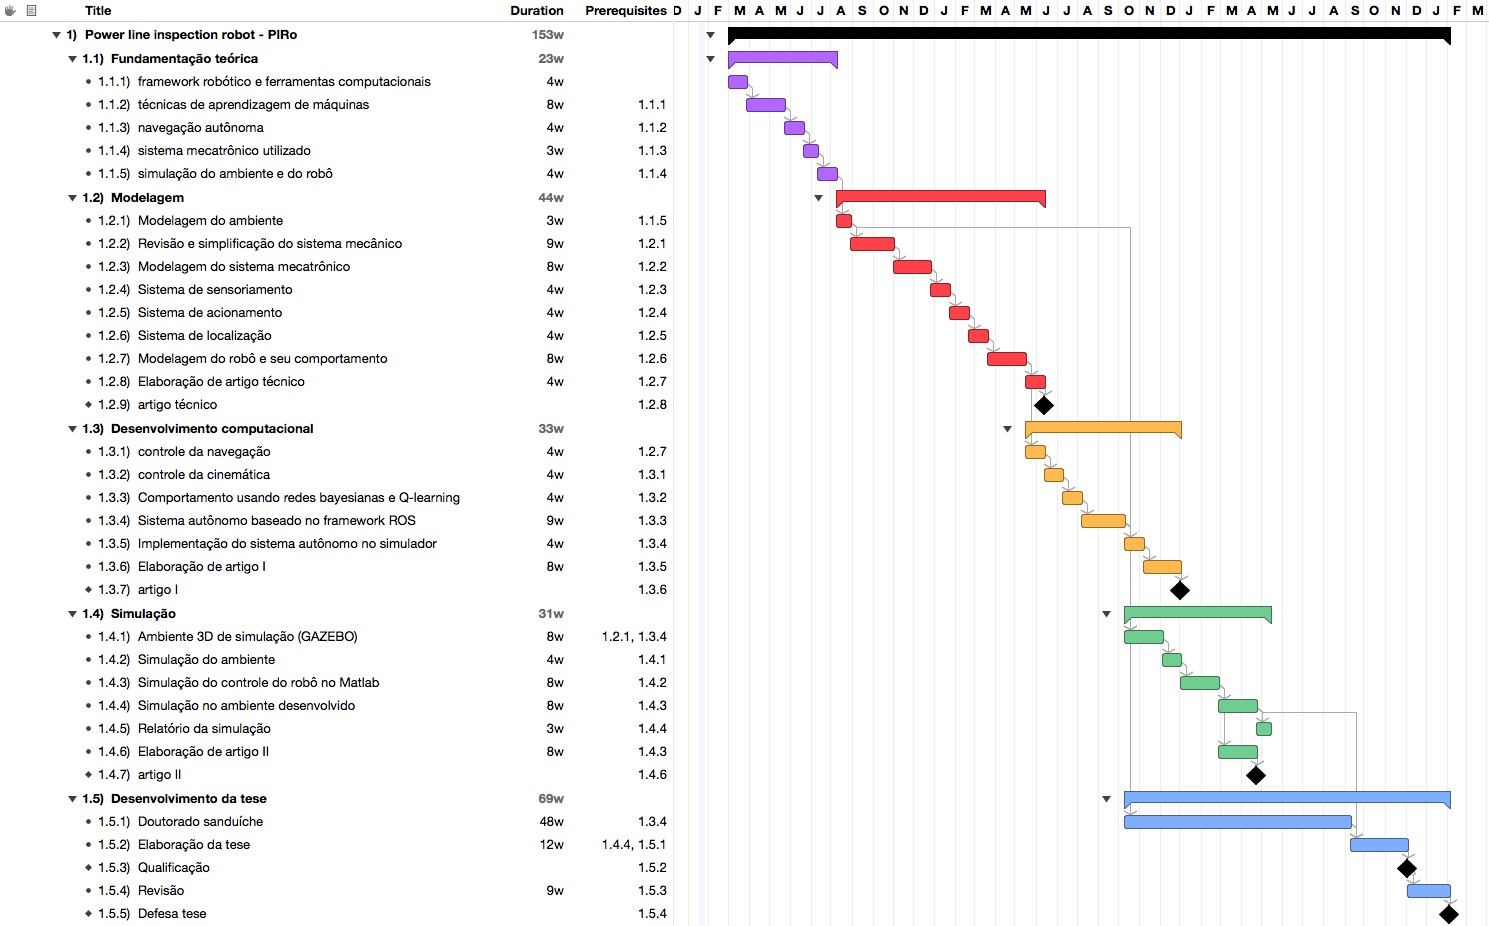
\includegraphics[width=1.1\textwidth]{./PIRo}				% Including picture
	\caption{Cronograma de atividades para o doutorado.}			% Including title
	\label{piro}												% Caption of the figure
\end{figure}													% End of the figure
%%%%

\noindent Para maiores detalhes é apresentado também a Tabela \ref{table:tasks1} com as sub-tarefas necessárias para a realização do projeto.

%%%%%%%%%%%%%%%%%%%% TABLE %%%%%%%%%%%%%%%%%%%%%%%%%%%%%%%
\begin{table} [ht!]
\caption{Principais atividades do projeto de tese.}
\centering
\begin{tabular}{p{0.3\linewidth}cp{0.5\linewidth}}
\hline\hline
Etapa & Duração & Atividades \\ [0.5ex] % inserts table %heading
\hline
Fundamentação teórica & 23 semanas & framework robótico e ferramentas computacionais; técnicas de aprendizagem de máquinas; navegação autônoma; sistema mecatrônico utilizado; simulação do ambiente e do robô\\
\hline
Modelagem & 44 semanas & modelagem do ambiente; revisão e simplificação do sistema mecânico; modelagem do sistema mecatrônico; sistema de sensoriamento, sistema de acionamento, sistema de localização, modelagem do robô e seu comportamento; elaboração de artigo técnico\\[1ex]
\hline
Desenvolvimento computacional & 33 semanas & controle da navegação; controle da cinemática; comportamento usando redes bayesianas e Q-learning; sistema autônomo baseado no ROS; implementação do sistema autônomo no simulador; elaboração de artigo I\\[1ex]
\hline
Simulação & 31 semanas & ambiente 3D de simulação; simulação do ambiente; simulação do controle do robô; simulação no ambiente desenvolvido; relatório da simulação; elaboração de artigo II\\[1ex]
\hline
Desenvolvimento da tese & 69 semanas & doutorado sanduíche; elaboração da tese; revisão\\[1ex]
\hline
\\
\end{tabular}
\label{table:tasks1}
\end{table}

\noindent Diante do exposto acima, o projeto terá as cinco partes desenvolvidas ao longo de 3 anos de desenvolvimento, com a fase de Desenvolvimento da tese e da Simulação iniciando-se paralelamente. Sugere-se o desenvolvimento de um período de um ano em uma instituição de renome para a realização de um Doutorado Sanduíche. A Universidade de Bremen localizada em Bremen na Alemanha desempenha uma boa referência no quesito robótico; como resultado de sua ação, no campus da universidade várias empresas do setor estão instaladas no intuito de desenvolver tecnologia de ponta para a indústria emergente da robótica.



